\documentclass[11pt]{article}
% arXiv 统计论文常见的 article + natbib 组合；投稿前应替换为目标期刊模板。
\usepackage[round,authoryear]{natbib}
\usepackage[margin=1in]{geometry}
\usepackage{graphicx}
\usepackage{booktabs}
\newcommand{\SampleSize}{32}
\newcommand{\ModelRsquared}{0.827}
\newcommand{\WeightEstimate}{-3.878}

\title{A Reproducible Statistical Workflow}
\author{Course example}
\date{}
\begin{document}
\maketitle
\section{Introduction}
Reproducible analysis benefits from explicit computational records \citep{wickham2014}
and transparent statistical reporting \citep{gelman2020}.
\section{Results}
The teaching analysis uses \SampleSize{} observations and has $R^2=\ModelRsquared$.
\begin{table}[h]
\centering
\caption{Model coefficients generated by R.}
\begin{tabular}{lrrrr}
\hline
Term & Estimate & SE & 95\% CI & $p$ \\
\hline
Intercept & 37.227 & 1.599 & [33.957, 40.497] & $<0.001$ \\
Weight (1000 lbs) & -3.878 & 0.633 & [-5.172, -2.584] & $<0.001$ \\
Horsepower & -0.032 & 0.009 & [-0.050, -0.013] & 0.001 \\
\hline
\end{tabular}

\end{table}
\begin{figure}[h]
\centering
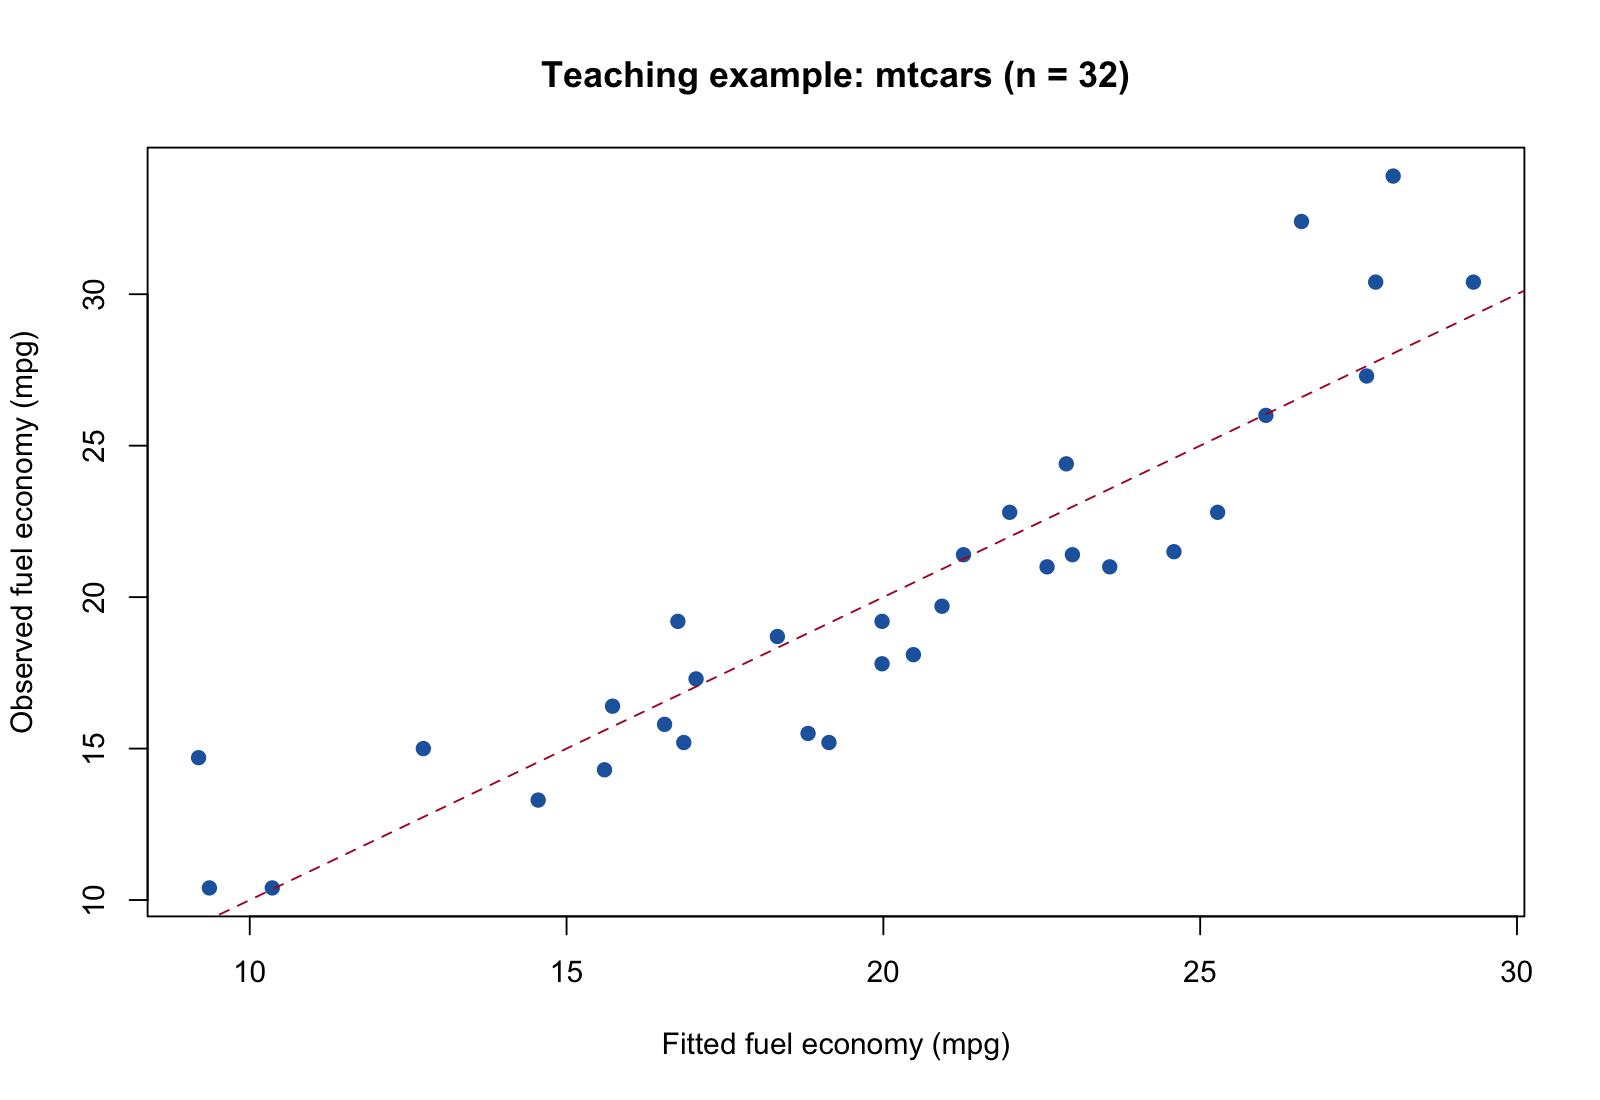
\includegraphics[width=.8\linewidth]{../../../outputs/figures/observed-fitted.pdf}
\caption{Observed and fitted values.}
\end{figure}
\bibliographystyle{plainnat}
\bibliography{references}
\end{document}
